\documentclass[tikz,border=5mm]{standalone}
\usepackage{tikz}
\usetikzlibrary{arrows.meta,positioning,fit,calc,backgrounds}
\begin{document}
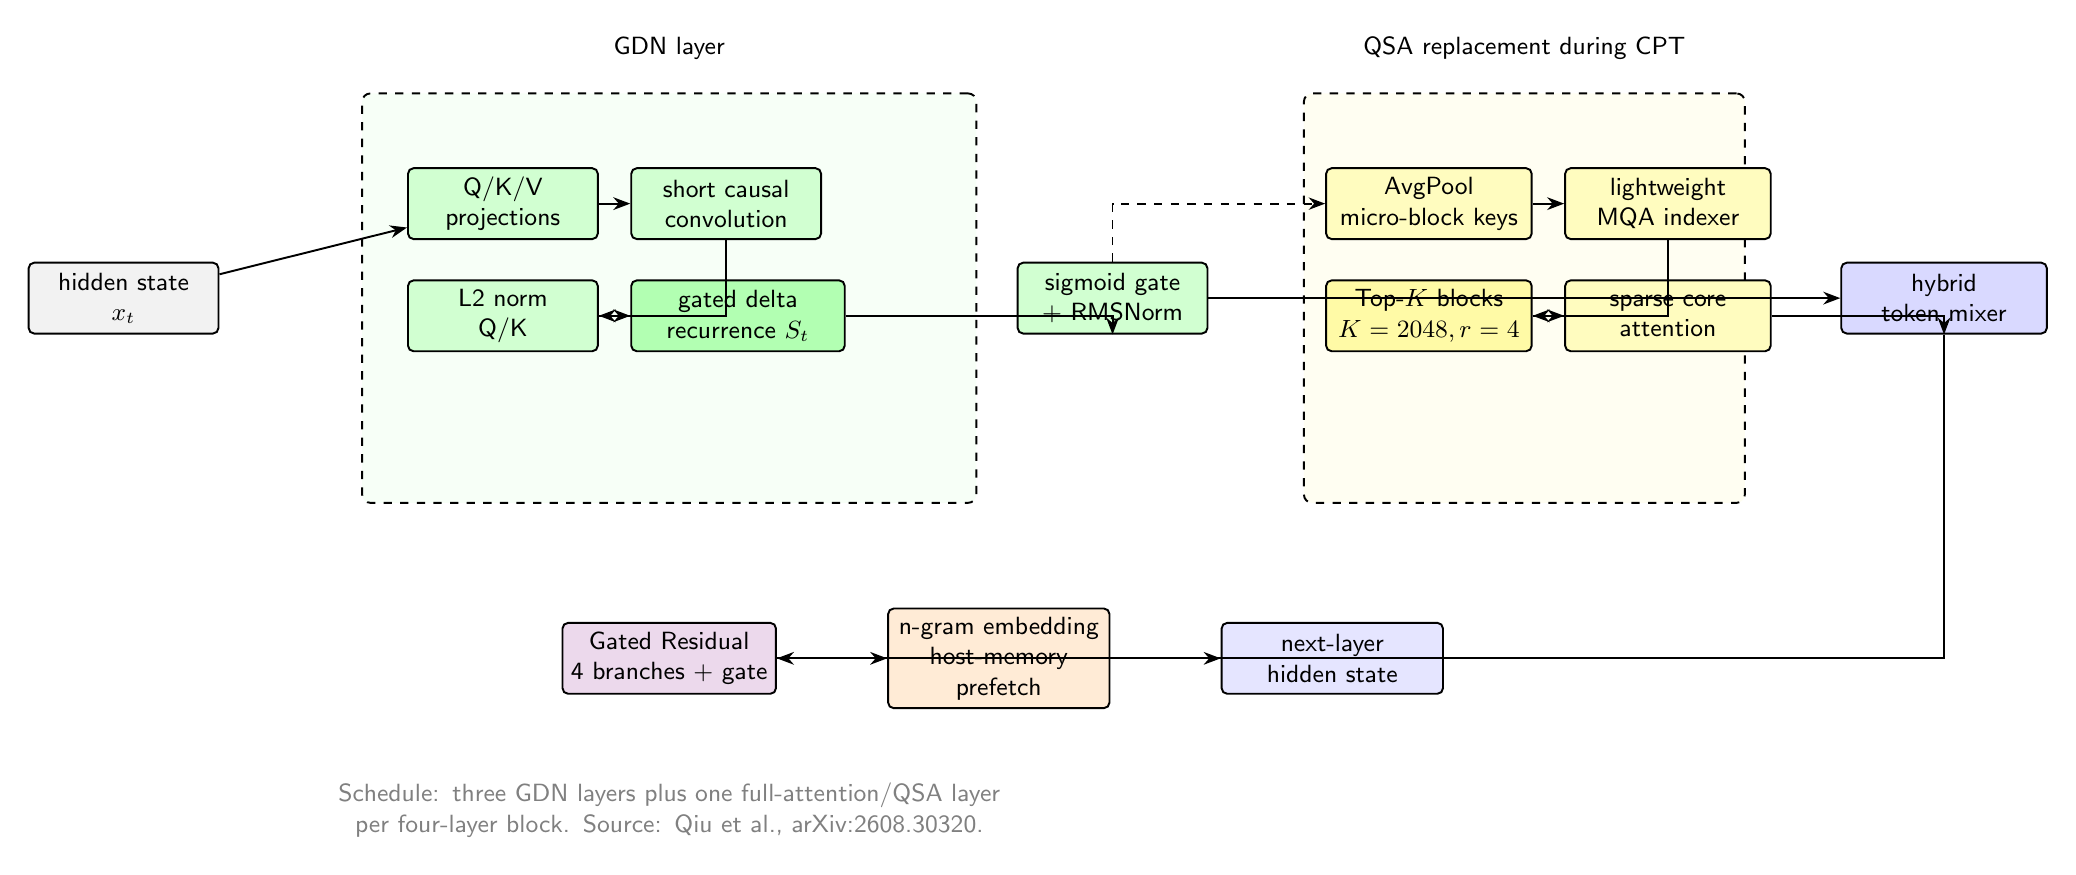
\begin{tikzpicture}[
  font=\sffamily\small,
  >=Stealth,
  box/.style={draw, rounded corners=2pt, minimum height=9mm, inner sep=3pt, align=center, line width=.7pt},
  flow/.style={-Stealth, line width=.7pt},
  aux/.style={-Stealth, dashed, line width=.65pt},
  group/.style={draw, rounded corners=3pt, dashed, inner sep=7pt, line width=.7pt}
]
\node[box, fill=gray!10, text width=22mm] (x) {hidden state\\$x_t$};
\node[group, fill=green!3, right=18mm of x, minimum width=78mm, minimum height=52mm] (gdn-group) {};
\node[box, fill=green!18, text width=22mm] at ($(gdn-group.west)+(18mm,12mm)$) (proj) {Q/K/V\\projections};
\node[box, fill=green!18, text width=22mm, right=4mm of proj] (conv) {short causal\\convolution};
\node[box, fill=green!18, text width=22mm, below=5mm of proj] (norm) {L2 norm\\Q/K};
\node[box, fill=green!30, text width=25mm, right=4mm of norm] (delta) {gated delta\\recurrence $S_t$};
\node[box, fill=green!18, text width=22mm, right=5mm of gdn-group] (gdn-out) {sigmoid gate\\+ RMSNorm};
\node[group, fill=yellow!5, right=12mm of gdn-out, minimum width=56mm, minimum height=52mm] (qsa-group) {};
\node[box, fill=yellow!25, text width=24mm] at ($(qsa-group.west)+(16mm,12mm)$) (compress) {AvgPool\\micro-block keys};
\node[box, fill=yellow!25, text width=24mm, right=4mm of compress] (indexer) {lightweight\\MQA indexer};
\node[box, fill=yellow!35, text width=24mm, below=5mm of compress] (topk) {Top-$K$ blocks\\$K=2048,r=4$};
\node[box, fill=yellow!25, text width=24mm, right=4mm of topk] (sparse) {sparse core\\attention};
\node[box, fill=blue!15, text width=24mm, right=12mm of qsa-group] (mix) {hybrid\\token mixer};
\node[box, fill=violet!15, text width=25mm, below=15mm of gdn-group] (gr) {Gated Residual\\4 branches + gate};
\node[box, fill=orange!16, text width=26mm, right=14mm of gr] (ngram) {n-gram embedding\\host-memory prefetch};
\node[box, fill=blue!10, text width=26mm, right=14mm of ngram] (out) {next-layer\\hidden state};

\draw[flow] (x) -- (proj);
\draw[flow] (proj) -- (conv);
\draw[flow] (conv) |- (norm);
\draw[flow] (norm) -- (delta);
\draw[flow] (delta) -| (gdn-out);
\draw[flow] (gdn-out) -- (mix);
\draw[flow] (mix) |- (gr);
\draw[flow] (gr) -- (ngram);
\draw[flow] (ngram) -- (out);
\draw[aux] (gdn-out) |- (compress);
\draw[flow] (compress) -- (indexer);
\draw[flow] (indexer) |- (topk);
\draw[flow] (topk) -- (sparse);
\draw[flow] (sparse) -| (mix);

\node[above=3mm of gdn-group] {GDN layer};
\node[above=3mm of qsa-group] {QSA replacement during CPT};
\node[below=10mm of gr, text width=150mm, align=center, text=gray] {Schedule: three GDN layers plus one full-attention/QSA layer per four-layer block. Source: Qiu et al., arXiv:2608.30320.};
\end{tikzpicture}
\end{document}
